\documentclass[10pt,a4paper]{report}

\usepackage[utf8]{inputenc}
\usepackage{amsmath}
\usepackage{amsfonts}
\usepackage{amssymb}
\usepackage{graphicx}
\usepackage{color}
\usepackage{enumitem}
\usepackage[top=1cm, bottom=2cm, left=2cm, right=2cm]{geometry}

\usepackage{fancyhdr}
\pagestyle{fancy}

\fancyhead{}
\fancyfoot{} 
\lhead{
\includegraphics{../Logo/logoKNKMini.jpg} \hspace{0.1cm} Kould Not Konect  \hspace{0.4cm} \vline}
\chead{Document de Conception Générale}
\rhead{Kould Not Share}
\rfoot{\thepage}

\author{Kevin BASCOL, Kevin LAOUSSING, Nicolas REYNAUD}
\title{Document de conception générale}
\date{3 Novembre 2014}

\makeatletter
\renewcommand{\thesection}{\@arabic\c@section}
\makeatother

\begin{document}

\makeatletter
	\begin{titlepage}
	
	\begin{figure}
		\begin{minipage}[c]{.46\linewidth}
		\end{minipage} \hfill
		\begin{minipage}[c]{.20\linewidth}
			\begin{center}
				
\includegraphics{../Logo/logoKNK.jpg}\\
				{\large Kould Not Konect}
			\end{center}
		\end{minipage}
	\vspace{1cm}
	\end{figure}
	
	\centering
		{
		\hrule height 2pt
		\vspace{0.7cm}
		\Huge \textbf{\@title}}\\
		\vspace{0.7cm}
		\hrule height 2pt
		\vspace{1.5cm}
		{\LARGE  Projet \textbf{Kould Not Share} v1.0}
		
		\vfill
		
		\begin{tabular}{|c|c|c|}
			\hline
			Version & Date & Description\\
			\hline
			V.1 & 16/11/14 & Première version de la conception générale\\
			\hline
			 & & \\
			\hline
			 & & \\
			\hline
		\end{tabular}\\
		\vspace{1cm}
		\@author\\
		\end{titlepage}
\makeatother
\setcounter{secnumdepth}{5}
\setcounter{tocdepth}{5}
\renewcommand{\contentsname}{Sommaire}
\begingroup\makeatletter
\def\@makeschapterhead#1{%
  {\parindent \z@ \raggedright
    \normalfont
    \interlinepenalty\@M
    \Huge \bfseries  #1\par\nobreak
    \vskip 20pt% <---- à réduire pour avoir plus de place
  }}\makeatother
\tableofcontents
\endgroup
\thispagestyle{empty}
\setcounter{page}{0}
\newpage

\newgeometry{top=2cm, bottom=2cm, left=2cm, right=2cm}

\section{Introduction}


\subsection{Portée du document}
Le logiciel de client/serveur FTP est un outil permettant à des particuliers ou des entreprises l'échange des données de manière contrôler. Par exemple, chaque utilisateurs propriétaires d'un fichier stocké dans le serveur FTP du logiciel, pourront paramétrer les droits de téléchargements sur ce fichier, et ainsi ils disposeront du pouvoir de restreindre ou d'augmenter l'accessibilité de son fichier...

\subsection{Objectif du document}
\begin{flushleft}
Ce document présente la conception logicielles et matérielles de la version 1.0 du projet Kould Not Share de l'entreprise Kould Not Konnect. Les responsables de ce projet sont Nicolas Reynaud, Kevin Laoussing et Kevin Bascol.
\end{flushleft}

\subsection{Définitions, acronymes et abréviations}
\begin{description}
\item[KNK] Kould Not Konect.
\item[KNS] Kould Not Share.
\item[FTP] File Transfer Protocol, protocole de communication destiné à l'échange informatique de fichiers sur un réseau TCP/IP.
\item [MVC] : Modèle-Vue-Controleur, est un modèle destiné à répondre aux besoins des applications interactives en séparant les problématiques liées aux différents composants au sein de leur architecture respective.
\item[Protocole] Spécification de plusieurs règles pour un type de communication particulier.
\item[Client] Logiciel qui envoie des demandes à un serveur.
\item[Serveur] Dispositif informatique matériel ou logiciel qui offre des services, à différents clients.
\item[Downloader] Anglicisme du mot "télécharger".
\item[Uploader] Anglicisme du mot "téléverser".
\end{description}

\section{Description générale}

Ce projet consiste en la création d'un serveur FTP chez un particulier ou une entreprise, ayant accès à la machine sur laquelle est installé le programme. Les utilisateurs se verront donner l'accès par l'administrateur à certains dossiers de la machine sur laquelle est installé le serveur. Il pourront faire alors des échanges de fichiers dans ces répertoires à l'aide du client FTP.\\

\section{Architecture du système Kould Not Share}

		Le logiciel Kould Not Share est composé en deux sous-système : le client et le serveur. Cette partie décrit la conception d'un point de vue modulaire et modèle, du logiciel KNS.
		
%		\begin{itemize}
%						\item Présenter les résultats renvoyés par le modèle.
%						\item Recevoir toute action de l'utilisateur (hover, clic de souris, sélection d'un bouton radio, cochage d'une case, entrée de texte, de mouvements, de voix, etc.).
%						\item Envoyer ces différents événements au contrôleur. 
%					\end{itemize}
					
%					\textbf{Ce module n'effectue pas de traitement, elle se contente d'afficher les résultats des traitements effectués par le modèle et d'interagir avec l'utilisateur.}\\
%				\end{flushleft}
    

	\subsection{Architecture modulaire du système}

		\subsubsection{Schéma de la décomposition modulaire du système}
			\begin{flushleft}
			Ce schéma présente d'une part le patron utilisé par le système et d'autre part la décomposition modulaire du système.\\
			Il décrit de manière général le fonctionnement du système à travers les interaction entre les modules.
			\end{flushleft}
			\begin{center}
				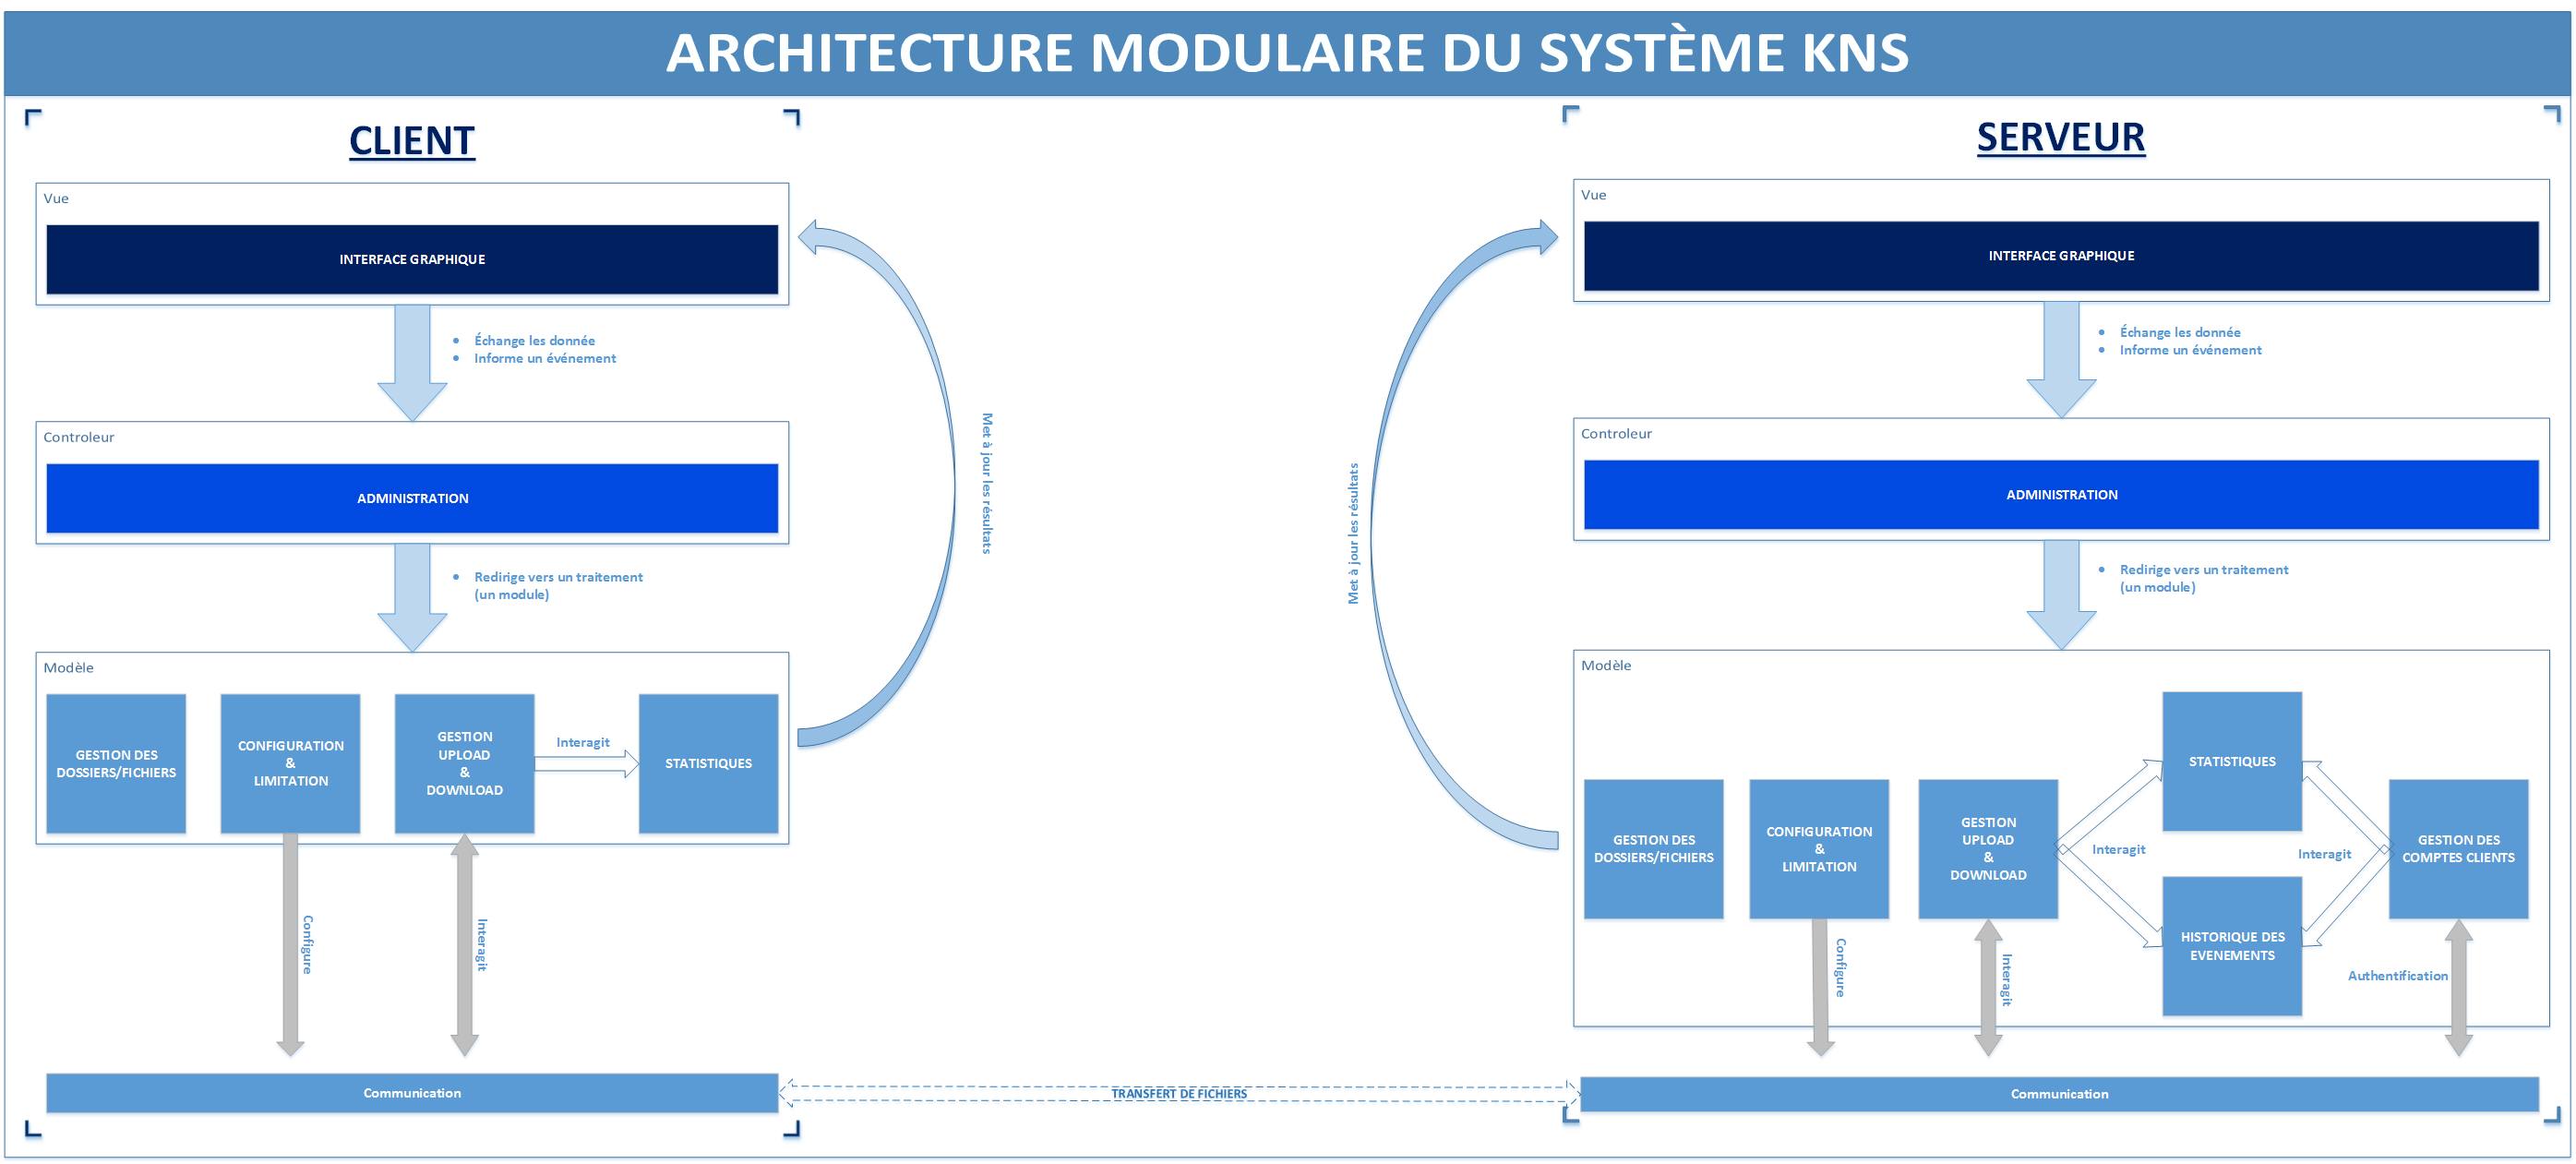
\includegraphics[scale=0.23]{Ressources/modules_KNS.png}
			\end{center}
		(cf Annexe.)

		\subsubsection{Description des modules}
		
			\paragraph{Modules Client}

				\subparagraph{Module interface graphique}
				\begin{flushleft}
				Le module de l'interface graphique contiendra toutes les classes Java implémentant l'interface graphique du client KNS. Le module utilisera principalement l'API Swing de la bibliothèque JFC. Il doit  accomplir les tâches suivantes :\\
					
					\begin{itemize}
						\item Présenter les informations,les données et les résultats renvoyés par un traitement.
						\item Recevoir toute action de l'utilisateur (hover, clic de souris, sélection d'un bouton radio, cochage d'une case, entrée de texte, de mouvements, de voix, etc.).
						\item effectuer correctement le traitement lié à l'événement. 
					\end{itemize}
					
					Ce module ne doit effectue pas de traitement, il doit se contenter d'afficher les résultats des traitements demandés par l'utilisateur.\\
				\end{flushleft}
						
				\subparagraph{Module d'administration}
				
				\begin{flushleft}
				Le module d'administration est l'ensemble des classes qui "administre" et coordonne les traitements selon les actions de l'utilisateur. de  il doit accomplir les tâches suivante:
				
				\begin{itemize}
					\item Prendre en charge la gestion des événements de synchronisation pour mettre à jour l'interface graphique selon le traitement effectué. 
					\item Recevoir tous les événements de l'interface graphique et enclencher les traitements à effectuer, autrement dit, enclencher le traitement d'un module.
				\end{itemize}
				
Ce module ne doit effectuer aucun traitement sur la requête de l'utilisateur. Il doit analyser l'action de l'utilisateur et se contenter d'appeler le traitement du module adéquat.
				\end{flushleft}
				
	
				\subparagraph{Module de gestion des dossiers}
				\begin{flushleft}
				Le module de gestion regroupe toutes les classes qui implémentent la gestion des dossiers. Ce module doit accomplir les tâches suivantes :
				\begin{itemize}
					\item les traitements de manipulation de fichiers et de répertoires (cf Document des spécifications des exigences, section 3.1.1.4).
					\item les traitements d'affichages (cf Document des spécifications des exigences, section 3.1.1.4).
				\end{itemize}
				
				Par conséquent le module doit interagir avec le système de l'utilisateur (manipulation de fichiers et de répertoires), et le module de communication (pour obtenir l'arborescence d'un répertoire héberger dans un serveur FTP).\\
				Le module ne doit effectuer de traitement que lorsqu'il est appelé par le module d'administration.
				\end{flushleft}
	
				\subparagraph{Module de configuration et limitation}	
				\begin{flushleft}
				Le module de configuration et limitation regroupe toutes les classes qui implémentent les configurations du client et les limitations des transferts de fichiers du module de communication (cf Document des spécifications des exigences, section 3.1.1.3).\\
				Le module doit interagir avec le module de communication pour lui appliquer la configuration décidée par l'utilisateur.\\
				Le module ne doit effectuer de traitement que lorsqu'il est appelé par le module d'administration.
				\end{flushleft}
	
				\subparagraph{Module de upload/download}
				\begin{flushleft}
				Le module de upload/download regroupe toutes les classes qui implémentent les opérations d'upload et de download d'un fichier (cf Document des spécifications des exigences, section 3.1.1.6). \\
				Le module doit interagir avec le module de communication et le systeme du client pour effectuer un transfert de fichiers(upload et download).\\
				Le module doit interagir avec le module de statistiques pour comptabiliser les opérations effectuées par le module de upload/download.\\
				Le module doit respecter la configuration donnée par le module de configuration et de limitation.
				Le module ne doit effectuer de traitement que lorsqu'il est appelé par le module d'administration.
				\end{flushleft}
	
				\subparagraph{Module de statistiques}
				\begin{flushleft}
				Le module de statistiques regroupe toutes les classes qui implémentent toutes les opérations de statistiques décrites dans le documents de  spécification des exigences (cf Document des spécifications des exigences, section 3.1.1.7).\\
				Le module doit effectuer des traitements à chaque opérations de transfert de donnée du module de upload/download, et lorsqu'il est appelé par le module d'administration.
				\end{flushleft}
				
	
				\subparagraph{Module de communication}
				\begin{flushleft}
				Le module de communication regroupe toutes les classes qui implémentent la communication de réseau. Le principale traitement de ce module est effectuer tout les types d'opérations réseau du logiciel. Ce module doit accomplir les taches suivantes :
				\begin{itemize}
					\item Permettre au client de se connecter à n'importe quel serveur FTP.
					\item Effectuer toutes les opérations d'authentifications (cf Document des spécifications des exigences, section 3.1.1.5).
					\item Effectuer toutes les opérations de transfert de fichier en respectant le protocle FTP et la configuration imposée le module de configurations et de limitations (cf Document des spécifications des exigences, section 3.1.1.6).
				\end{itemize}
				
				Le module doit interagir avec le module de upload/download lors d'un transfert de fichiers.\\
				\end{flushleft}
				
				
			\paragraph{Modules Serveur}
				Les modules du serveur reprend les même modules que le client, mais possède des modules supplémentaire.
				
				\subparagraph{Module des historiques des événements}
	
	
				\subparagraph{Module de gestion des comptes clients}

				
	\subsection{Modèle MVC}
		Notre logiciel utilise un modèle MVC pour la partie client et la partie serveur.
		\subsubsection{Rappel}
			
			\paragraph{Principe de MVC}
			\begin{flushleft}

			Le modèle MVC permet de bien séparer les données, la présentation et les traitements correspondant respectivement aux trois parties suivantes : le modèle, la vue et le contrôleur (voir section 1.1 Schéma du système).\\
Pour rappel, lorsqu'un utilisateur interagie avec l'interface graphique de l'application (qui correspond à la vue du patron MVC), celle-ci envoie une requête  :
				\begin{itemize}
					\item la requête envoyée depuis la vue est analysée par le contrôleur (par exemple un clic de souris pour lancer un traitement de données) ;
    				\item le contrôleur demande au modèle approprié d'effectuer les traitements et notifie à la vue que la requête est traitée ;
    				\item la vue notifiée fait une requête au modèle pour se mettre à jour (par exemple affiche le résultat du traitement "via" le modèle).

				\end{itemize}
			\end{flushleft}
			
		\paragraph{La vue}
			\subparagraph{Description}
			\begin{flushleft}
				Elle fournit une présentation du modèle. En général, la vue reçoit directement du modèle l’état et les données qu’elle doit afficher.
			\end{flushleft}
			
			\subparagraph{Modules composant la vue de MVC}
			\begin{flushleft}
				\begin{itemize}
				 	\item Module de l'interface graphique.
				\end{itemize}
			\end{flushleft}
			
		\paragraph{Le contrôleur}
			\subparagraph{Description}
			\begin{flushleft}
				Il accepte les entrées des utilisateurs et détermine ce qu’elles
signifient pour le modèle.
			\end{flushleft}
			
			\subparagraph{Modules composant le contrôleur de MVC}
			\begin{flushleft}
				\begin{itemize}
					\item Module administration.
				\end{itemize}
			\end{flushleft}
			
		\paragraph{Le modèle}
			\subparagraph{Description}
			\begin{flushleft}
				Le modèle contient les états, les données et la logique applicative. Il n’a pas conscience de la vue ni du contrôleur, même s’il fournit une interface pour accéder à son état et le manipuler et s’il peut informer les observateurs des changements d’état.
			\end{flushleft}
			
			\subparagraph{Modules composant le modèle de MVC}
			\begin{flushleft}
			Pour la partie client :
				\begin{itemize}
					\item Module de gestion de dossiers/fichiers;
					\item Module de configuration et limitation;
					\item Module de gestion de upload/download;
					\item Module de statistiques;
				\end{itemize}
			Pour la partie serveur :
			\begin{itemize}
					\item Module de gestion de dossiers/fichiers;
					\item Module de configuration et limitation;
					\item Module de gestion de upload/download;
					\item Module de statistiques;
					\item Module de gestion des comptes clients;
					\item Module de gestion des historiques des événements.
				\end{itemize}
			\end{flushleft}

			
		\subsubsection{Conception du modèle MVC}
		
		Le modèle MVC est un patron de conception composé : il intègre plusieurs patrons de conceptions décrite dans cette section.
		
		\paragraph{Observateur}
		\begin{flushleft}
				Le modèle implémente le patron de conception Observateur, afin que les objets intéressés soient mis à jour quand un changement d’état se produit. L’emploi du patron de conception Observateur garantit que le modèle demeure complètement indépendant des vues et des contrôleurs. Il permet également d’utiliser des vues différentes avec le même modèle, voire d’en utiliser plusieurs en même temps.

		\end{flushleft}
		\paragraph{Stratégie}
		\begin{flushleft}
		La vue et le contrôleur mettent en œuvre le patron de conception Stratégie : la vue est un objet qui est configuré avec une stratégie. Le contrôleur fournit la stratégie. La vue n’est concernée que par les aspects visuels de l’application et délègue au contrôleur toutes les décisions sur le  comportement de l’interface. L’emploi du pattern Stratégie permet également de découpler la vue du modèle parce que c’est le contrôleur qui a la responsabilité d’interagir avec le modèle pour exécuter les requêtes des utilisateurs. La vue ne sait absolument pas comment il procède.		
		\end{flushleft}



\section{Définition des principales structures de données}

	\subsection{Structures de données}

	\subsection{Interactions entre les structures de données} %<--- diagramme de séquence ?%

\newpage
\section{Annexe}

\subsection{Architecture modulaire du système KNS}
	\begin{center}
	\rotatebox{270}{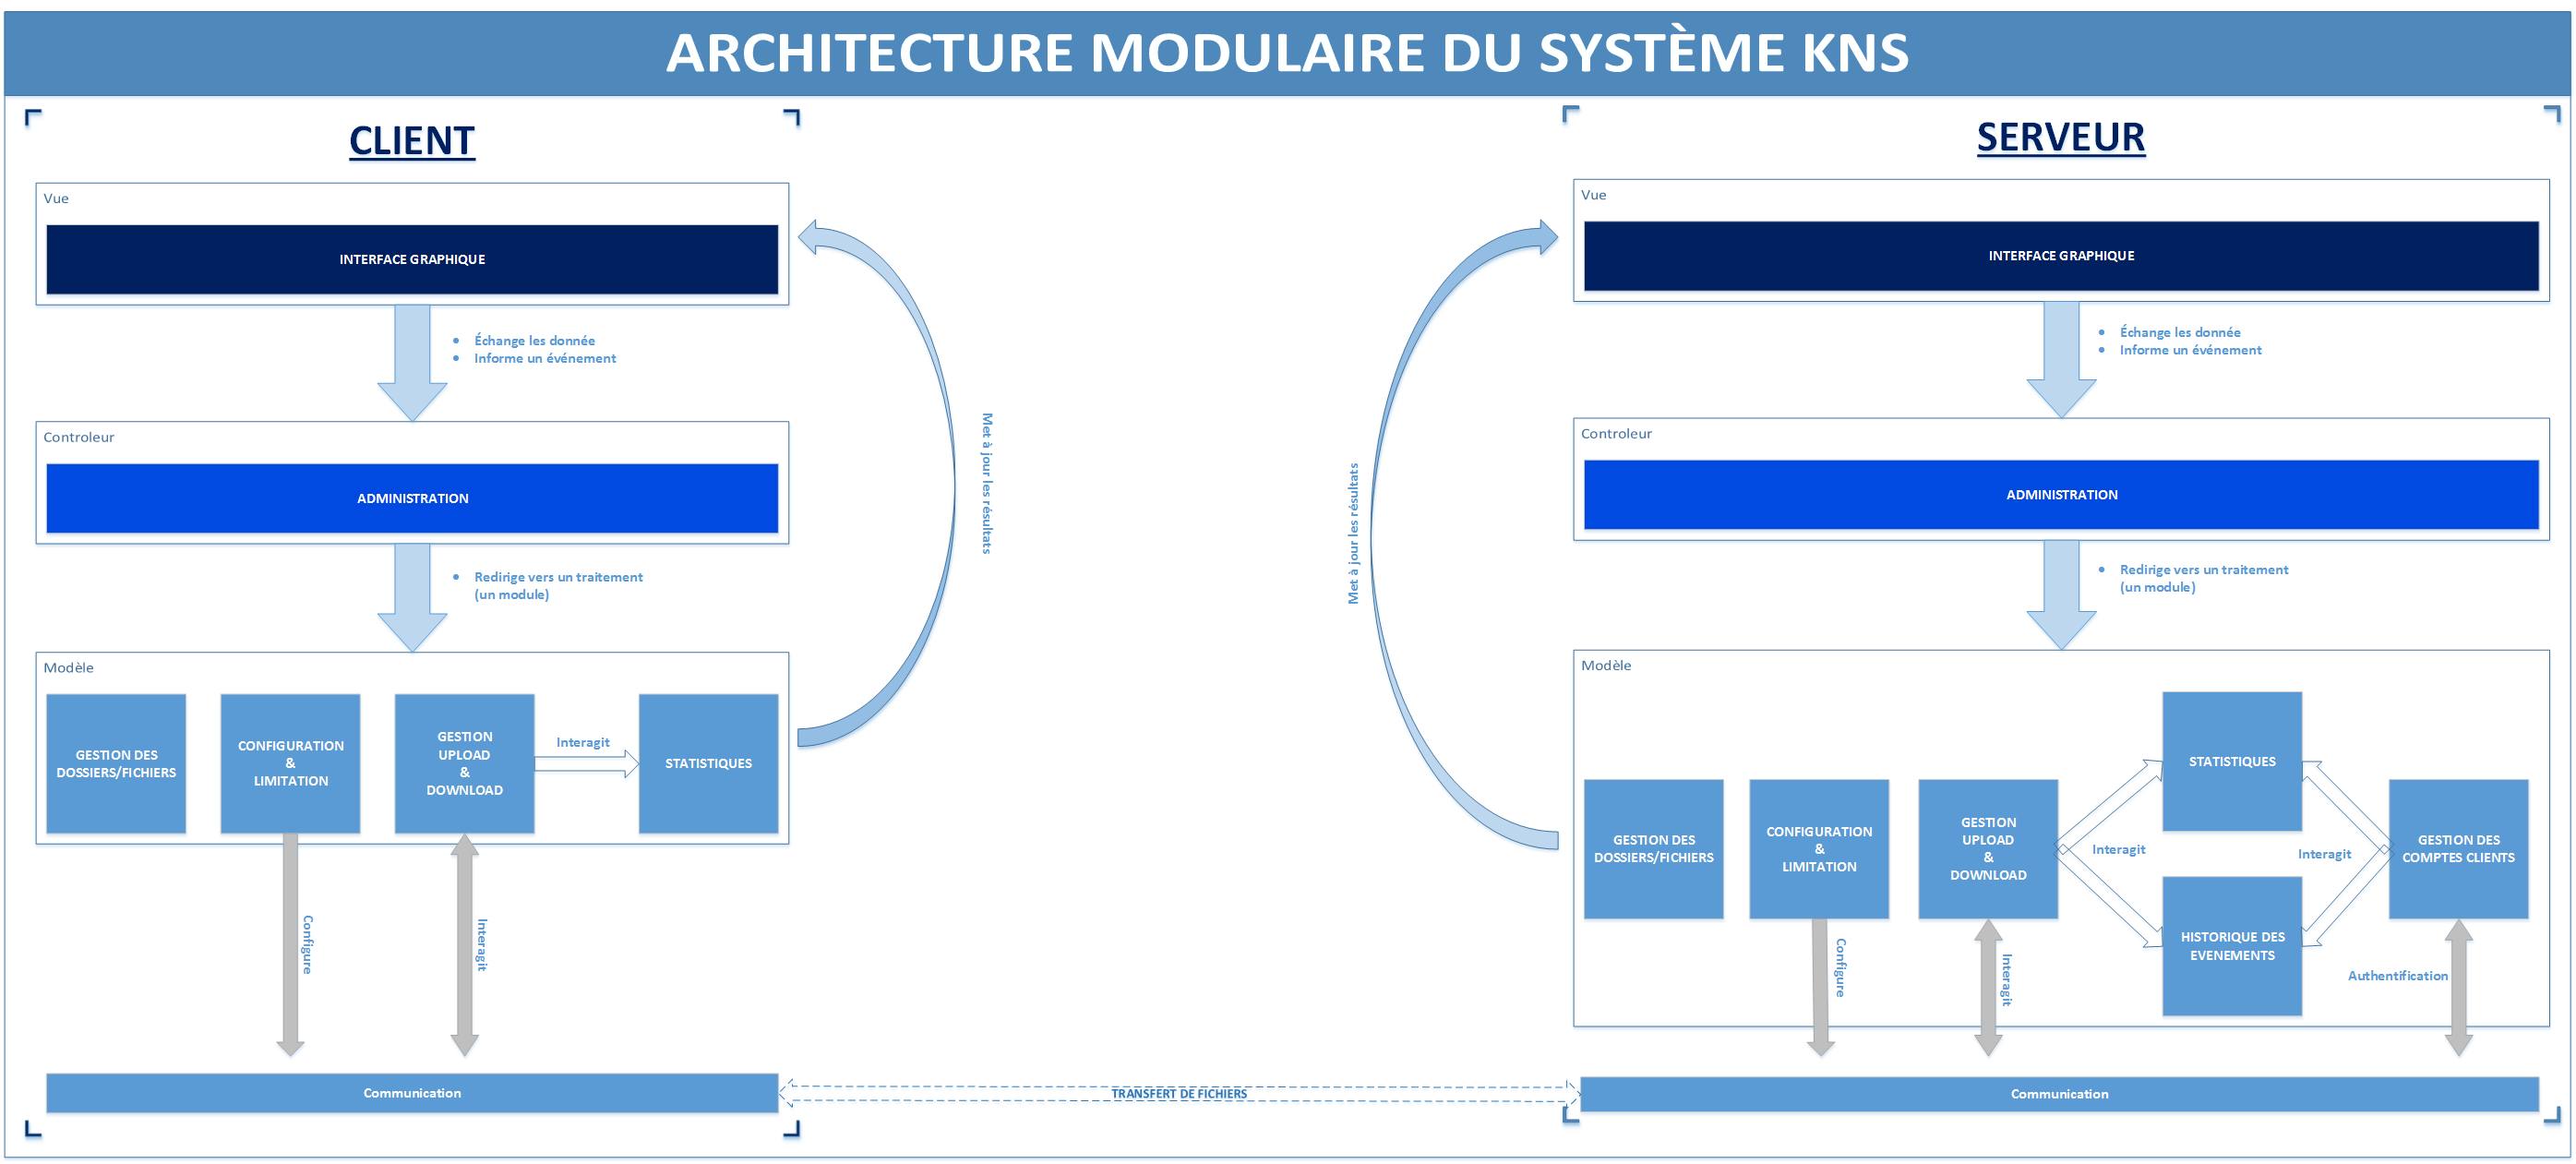
\includegraphics[scale=0.35]{Ressources/modules_KNS.png}}	
	\end{center}
\end{document}